\section{Introduction}
\label{sec:intro}

Multi-step relational visual reasoning requires a multimodal large language model (MLLM) to sequentially locate and inspect a chain of distinct objects across cluttered scenes. Standard textual chain-of-thought (CoT) prompting struggles to serialize fine-grained spatial coordinates without loss of geometric precision~\cite{shao2024visualcot,wu2024vstar}, whereas iterative pixel-cropping pipelines incur repeated visual re-encoding overhead~\cite{su2025pixelreasoner,zheng2026deepeyes}. Continuous latent visual reasoning offers a third paradigm: inspired by continuous thought in language models~\cite{hao2025coconut,shen2025codi}, methods such as Latent Visual Reasoning (LVR)~\cite{li2026lvr}, Mirage~\cite{yang2026mirage}, and Monet~\cite{wang2026monet} autoregressively feed last-layer hidden states back as input embeddings $H_{1:L} = (h_1, \dots, h_L)$ between boundary tokens (\texttt{<|lvr\_start|>} and \texttt{<|lvr\_end|>}), supervising them to reconstruct Region-of-Interest (ROI) visual patch features prior to text generation.

\begin{figure*}[t]
  \centering
  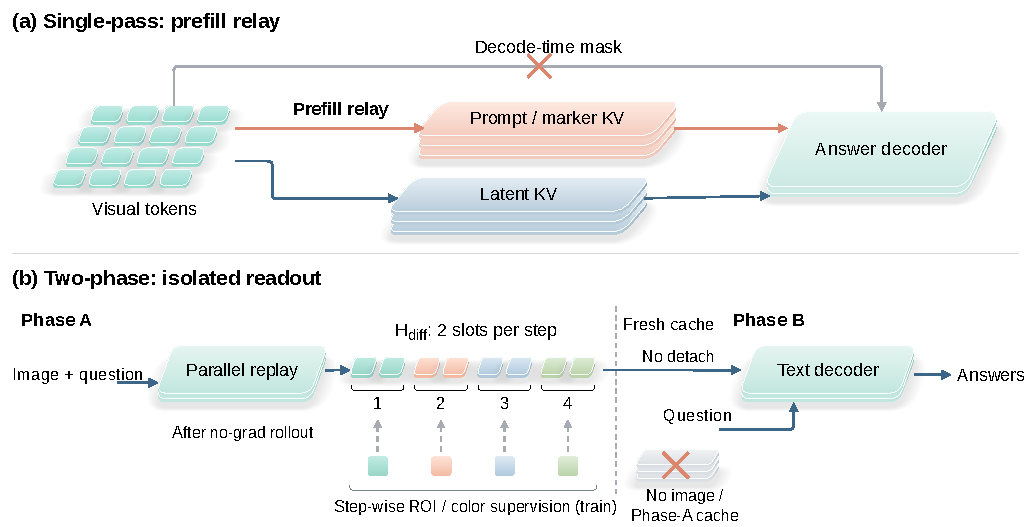
\includegraphics[width=0.78\textwidth]{figs/fig1_teaser_overview.pdf}
  \caption{\textbf{Cached Visual Routes, Across-Layer Interventions, and Isolated Readout.} \textbf{(a)} The image conditions both cache partitions during prefill; a decode-time visual-key mask leaves both cached routes accessible. \textbf{(b)} Each sheet shows KV caches at one layer; dashed columns select the same partition through all $28$ layers. \texttt{C3a/b} and \texttt{C2} are donor swaps on the adapted \texttt{E5} checkpoint (\texttt{C3a} swaps prompt/start caches and recomputes $\Mend$; \texttt{C3b} also transplants $\Mend$'s cache) under visual-key masking at $\Mend$ and answer readout. Rates use eligible subsets; zero flips do not establish image-independent latent caches. \textbf{(c)} Phase A rolls out $H_{\mathrm{raw}}$ without gradients, then uses parallel teacher-forced replay to emit $H_{\mathrm{diff}}$. Following prior isolation principles~\cite{li2026livr,park2026cvrr}, Phase B recomputes all layers from $H_{\mathrm{diff}}$, the question, and markers without image tokens or Phase-A KV, flowing answer-loss gradients through the non-detached tape into replay. Donor swaps interpolate the edited step's two slots ($m=2$, $K=4$ shown).}
  \label{fig:teaser}
\end{figure*}

Recent single-hop studies have scrutinized whether latent states genuinely mediate visual reasoning~\cite{li2026capimagine,guo2026beyond,li2026livr,park2026cvrr,realvr2026}. Perturbations on Monet and Mirage yield minimal single-hop loss~\cite{li2026capimagine}, and decomposing the latent span into slot contents, boundary markers, and format shows that image-conditioned slot contents do not act as portable visual memories when the image remains accessible ($|\text{Normal} - \text{ZeroSlot}| \le 2.7$pp, with marker-only decoding $L=0$ recovering $78\%$--$100\%$ of single-hop gains)~\cite{guo2026beyond}. Architecturally, LIVR~\cite{li2026livr} shows that single-pass learnable bottleneck tokens require masking both prompt-to-vision and answer-to-vision attention in Stage 1, while CVRR~\cite{park2026cvrr} shows that layer-20 multimodal question states retain $99\%$ of single-hop competence ($75.4\%$ vs.\ $75.9\%$ on V*) and that removing original multimodal caches under a strict readout interface (\texttt{w/o Bypass}) collapses six latent reasoners (including \texttt{LVR-7B}) to $35.6\%$. Meanwhile, ReaLVR~\cite{realvr2026} identifies the detached-replay gradient gap in LVR's Stage-2 GRPO and aligns all slots toward a single pooled visual prototype $p^+$.

Building on these single-hop diagnostics and visual-isolation precedents~\cite{guo2026beyond,li2026livr,park2026cvrr}, we investigate \textbf{single- and multi-step relational tracking ($K \in \{1, 2, 4\}$) with explicit autoregressive slot rollouts} across three questions:
(1) \emph{Are native continuous latent slots neutral on distractor-rich relational scenes across $K \in \{1, 2, 4\}$ under intact delimiters?}
(2) \emph{Under step-wise supervision and decoding-time vision masking, how do all-layer latent KV caches ($\KV_H$) versus prefill caches ($\KV_{Q,M}$) mediate predictions?}
(3) \emph{Under a strict image-free interface, what trade-offs govern step-aligned sub-windows, prior calibration, auxiliary supervision, and recurrent slot emission?}

A census of $123,287$ images in COCO~\cite{lin2014coco} shows that natural photos virtually never simultaneously satisfy non-degenerate $K=4$ color transitions and same-color distractor constraints ($M_{\mathrm{dist}} \ge 2$). We construct a controlled benchmark of $50$ dev and $150$ disjoint frozen evaluation clusters, paired with $87$ unseen-color counterfactual pairs ($266$ records), $496$ verified in-vocabulary recoloring records, and $600$ implicit pointer-chaining queries. Across seven modules totaling over $200,000$ passes on \texttt{LVR-7B}~\cite{li2026lvr} and its adapted variants (\cref{fig:teaser}), we establish three contributions:

\textbf{1. Destructive Slot Interference Across $K \in \{1, 2, 4\}$ (\texttt{E3-C}, \texttt{E7-2}).} Across the $150$ frozen clusters, native rollouts degrade $K=2, 4$ chain accuracy by $10.33$--$19.67$pp (\texttt{E3-C}, $9,600$ runs) and already degrade single-hop $K=1$ accuracy on the exact same scenes by $16.00$--$21.67$pp (\texttt{E7-2}, $13,200$ outputs), refuting slot neutrality on distractor-rich scenes. Boundary markers alone are neutral ($\pm 0.67$pp vs.\ \texttt{NoLatent}), whereas zeroing slot inputs (\texttt{Zero-Slot}) recovers $100\%$ of \texttt{NoLatent} accuracy (Proposition~\ref{prop:margin}).

\textbf{2. 28-Layer KV Double Dissociation Under Decoding-Masked Adaptation (\texttt{E3-B}, \texttt{E5}, \texttt{E6-C}).} While single-turn recoloring flips \texttt{LVR-7B} predictions on $61.90\%$--$72.09\%$ of queries ($\|\Delta H\|_2 = 69.25$) and local visual patch swaps (\texttt{E3-B1}) flip $83.93\%$--$93.75\%$ of eligible answers, donor latent patching yields $0.00\%$ flips and flat logit slopes ($\delta M(1) \in [-0.095, -0.011]$, \texttt{E3-B2}). Adapting \texttt{LVR-7B} with step-wise supervision and $60\%$ decoding-time vision masking (\texttt{E5}) raises vision-masked accuracy to $67.00\%$--$85.33\%$ with $0.00\%$ donor flips; 28-layer KV swaps (\texttt{E6-C}, Proposition~\ref{prop:bypass}) show $0.00\%$ flips from $\KV_H$ vs.\ $96.88\%$--$100.00\%$ on eligible pairs from $\KV_{Q,M}$ ($16.46\%$--$40.23\%$ full set), and $-64.00$ to $-73.00$pp under blind prefill.

\textbf{3. Step-Window Control, Prior Trade-Offs, and Recurrent Chaining Under Strict Isolation (\texttt{E6}, \texttt{E7}).} Under a LIVR/CVRR-style image-free interface (Proposition~\ref{prop:isolation}), step-aligned 2-slot windows (\texttt{E6-A}) achieve $82.00\%$--$83.33\%$ ($K=2$) and $72.67\%$--$75.67\%$ ($K=4$) chain accuracy on seen colors ($+63.67$ to $+69.00$pp over shared prototypes \texttt{E6-B}), driven synergistically by ROI-MSE ($38.33\%$--$41.00\%$) and Color-CE ($55.33\%$--$57.33\%$) over \texttt{Answer-CE Only} ($5.00\%$--$5.67\%$, \texttt{E7-3b}). On in-vocabulary recoloring (\texttt{E7-1a}), \texttt{E6-A} achieves $73.40\%/58.53\%$ full-set flips ($+70.19/+58.06$pp window specificity), while $K\times K$ logit matrices (\texttt{E7-3a}) quantify $k=r+1$ spillover (max off-diagonal $0.49$--$0.70$ log-odds). On held-out \texttt{yellow/brown}, narrow training priors limit raw \texttt{E6-A} flips to $0.00\%/3.12\%$, while prior calibration ($23.78\%/45.18\%$) and 8-color+KL training ($85.37\%/82.29\%$ new-color, $57.32\%/47.79\%$ joint flips) unlock unseen colors at a cost to original-image accuracy (\texttt{E7-1b}). Finally, on pointer chaining (\texttt{E7-4}), recurrent emission beats parallel emission by $+10.00$pp in strict readout ($80.67\%$ vs.\ $70.67\%$ on $K=2$; $41.33\%$ vs.\ $31.33\%$ on $K=4$), narrowing the gap to same-weight direct vision ($87.33\%/63.00\%$).
